%!TEX root = ../dokumentation.tex

\chapter{Grundlagen der Arbeit}

Im Folgenden werden die zu Grunde liegenden Technologien der Arbeit kurz erörtert.

\section{Raspberry Pi 3 Model B}
Ein \textit{Raspberry Pi} ist ein kleiner Minicomputer, welcher in etwa die
Größe einer Kreditkarte einnimmt. Seit der Erstveröffentlichung im Jahre 2011
hat sich am Grundkonzept des kleinen Computers nicht viel
geändert, lediglich die Anschlüsse sind mehr geworden und die verbauten
Prozessoren haben sich verbessert. 
Ein Grund für die weite Verbreitung der Minicomputer ist neben der kleinen
Größe auch der günstige Preis. So liegt der Preis des aktuellsten Modells bei
gerade einmal 30 Euro. Des Weiteren ist der Stromverbrauch sehr gering,
weshalb der Raspberry von den Benutzern auch oft als kleiner Server im Heimnetz
betrieben wird. Im Dauerbetrieb liegt der Jahresverbrauch beim neusten Raspberry
Pi's 3 Modell B bei etwa 53 kWh, was bei einem Preis von
circa 20 Cent pro kWh Gesamtkosten von 10 Euro pro Jahr bedeuten würde. \newline
Die Intention der Entwickler war es mit dem Raspberry Pi ein Gerät zu
entwerfen, welches Personen in jedem Alter die Möglichkeit bietet einen
Computer zu benutzen und programmieren zu lernen. Das Standard Betriebssystem
des Raspberry Pi basiert auf einer eigen entwickelten Linux Distribution mit
dem Namen \textit{Raspbian}.
\autocite{what_is_a_raspberry_pi?_2019}
\begin{figure}[h]
	\centering
	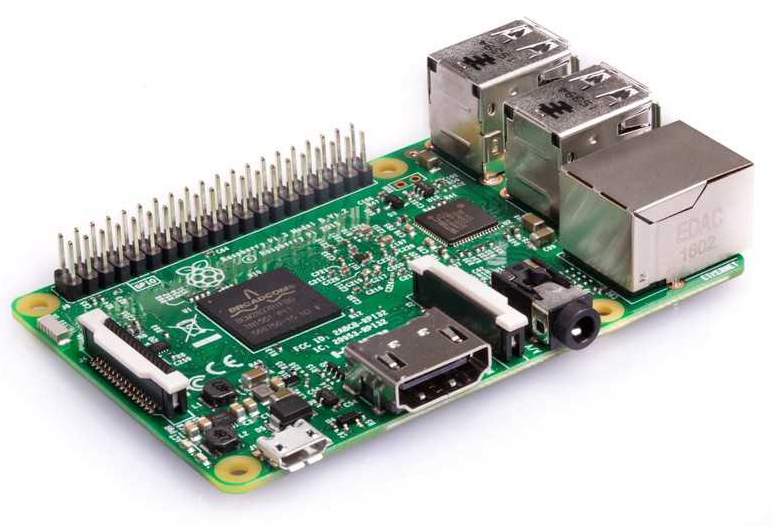
\includegraphics[scale=0.35]{Raspberry_Pi_3_Model_B.jpg}
	\caption{Beispielbild - Raspberry Pi 3 Model B \autocite{raspberry_pi_2019}}
	\label{img:grafik-RaspberryPi3}
\end{figure}
\newline

Auf dem in der Abbildung \ref{img:grafik-RaspberryPi3} dargestellten Raspberry
Pi handelt es sich um ein Gerät der neusten Generationen, den Raspberry Pi 3
Model B. Er zeichnet sich durch eine neue 64-Bit \ac{ARM}-\ac{CPU} mit 1.2
\ac{GHz} aus und besitzt dazu 1 \ac{GB} \ac{RAM}. Des Weiteren stellt er
sämtliche Anschlüsse wie z.B. 4 \ac{USB} Ports, RJ45 Anschluss, \ac{HDMI}
Anschluss sowie 40 \ac{GPIO} Ports zur Verfügung. Mit dem neusten Model des
Raspberry Pi wurde zudem noch eine \ac{WLAN} sowie Bluetooth Karte integriert.
In der Kombination mit dem \ac{SD-Karten} Slot, welcher als Speicher benutzt
wird, stellt der Raspberry Pi einen vollwertigen Computer dar.
\autocite{kurniawan_2016}
 
\section{Go}
\textit{Go} (oder auch \textit{Golang}) ist eine Programmiersprache, welche von
Robert Griesemer, Rob Pike und Ken Thompson (alles Mitarbeiter
von Google) entwickelt wurde. Ziel hinter Go war es eine effiziente und ausdrucksstarke Sprache zu entwickeln, welche es ermöglicht verlässliche und
leicht-leserliche Programme zu entwerfen \autocite{donovan_kernighan_2016}.
2009 wurde Go erstmals veröffentlicht, und wird seitdem von Google als Open Source
Software bereitgestellt. \newline
Im direkten Vergleich zu anderen Programmiersprachen reiht sich Go zwischen
C/C++ und Perl ein. Bei der Positionierung von Go setzt Google darauf, Go als
Sprache für Systemprogrammierung zu etablieren. Dabei setzt Google auf eher
untypische Mittel, da es in Go einen Garbage Collector gibt und zusätzlich eine
Unterstützung für Parallel- und Multicore-Verarbeitung
\autocite{feike_blass_2012}. \newline 
Gründe für die Beliebtheit von Go sind unter anderem die Einfachheit bei der
Entwicklung sowie die Geschwindigkeit bei der Kompilierung und
Ausführung von Programmcode. Zusätzlich besitzt Go ein integriertes Feature namens
\textit{Goroutinen}, welches Nebenläufigkeiten von Prozessen unterstützt und
deren Kommunikation über Kanal ermöglicht. 
Ein weiterer großer Vorteil ist, dass Go plattformübergreifend läuft. Das bedeutet,
dass Go-Programmcode ohne weitere Modifikation auf jedem gängigen Betriebssystem gleich
läuft.
\autocite{donovan_kernighan_2016}


\section{Git and GitHub}
Bei \textit{Git} handelt es sich aktuell um eines der bekanntesten
Versionskontrollsysteme. Entwickelt wurde es im Jahre 2005 von Linus Torvald,
der im Rahmen der Entwicklung des Linux-Kernels ein zufälliges System zur
Versionierung und Verwaltung seines Source Codes benötigte. Unter einem
Versionskontrollsystem wird im allgemeinen eine Software verstanden, welche
Änderungen des Programmcodes abspeichert und protokolliert. Dies birgt nicht nur
eine erhöhte Sicherheit bei der Entwicklung, da jeder gespeicherte Zustand
wiederhergestellt werden kann, sondern stellt gleichzeitig eine Art
Protokollierung des Programmcodes dar, da zusätzlich zu den verschiedenen
Programmzuständen weitere Informationen wie Autor, Zeitpunkt oder auch eine
kurze Beschreibung mit erfasst werden \autocite{preissel_stachmann_2017}. \hfill
\break 

Da Programme selten nur von einer Person an einem einzelnen PC entwickelt
werden, bietet Git nicht nur Möglichkeiten zur einfachen, sondern auch zur
verteilten Versionskontrolle. Um diese Verteilung optimal zu ermöglichen, haben
sich verschiedene Dienstleister wie \textit{GitHub} gebildet, welche einen
Service zum Hosten von Programmcode auf ihren Servern bereitstellen. Dadurch
haben Teams bzw. Nutzer einen zentralen Ort zur Speicherung des Programmcodes,
wodurch ein gleichzeitiges Arbeiten an einem Projekt ermöglicht wird. Des
Weiteren stellt GitHub noch weitere Funktionen zur Verfügung. So verfügt GitHub
neben dem reinen Ablegen von Programmcode noch über ein Web Interface, ein Wiki
oder auch ein Diskussionsbereich. Dies vereinfacht nochmals das dezentrale
Arbeiten von Teams an einem Projekt. Außerdem bietet GitHub Möglichkeiten zur
automatisierten Ausführung von \textbf{Hier fehlt iwas?!} Außerdem bietet GitHub Schnittstellen zu anderen
Tools wie beispielsweise \ac{CI}. So können über eine \ac{CI} automatisierte Abläufe
definiert werden, die beim Hochladen einer neuen Version des Programmcodes automatisierte Tests oder ähnliches vornehmen \autocite{bell_2014}.  

